%!TEX root = forallxyyc-solutions.tex
%\part{Interpretações}
%\label{ch.semantics}
%\addtocontents{toc}{\protect\mbox{}\protect\hrulefill\par}

\stepcounter{chapter} % Extensionality

\chapter{Verdade na LPO}\setcounter{ProbPart}{0}
\problempart
\label{pr.TorF1}
Considere a seguinte interpretação:
	\begin{itemize}
		\item O domínio contém apenas Corwin e Benedict
		\item $\atom{A}{x}$ é verdadeira para Corwin e Benedict
		\item $\atom{B}{x}$ é verdadeira apenas para Benedict
		\item $\atom{N}{x}$ não é verdadeira para ninguém
		\item $c$ refere-se a Corwin
	\end{itemize}
Determine se cada uma das seguintes sentenças é verdadeira ou falsa nessa interpretação:
\begin{compactlist}
\item $\atom{B}{c}$ \hfill \myanswer{Falso}
\item $\atom{A}{c} \eiff \enot \atom{N}{c}$ \hfill \myanswer{Verdadeiro}
\item $\atom{N}{c} \eif (\atom{A}{c} \eor \atom{B}{c})$ \hfill \myanswer{Verdadeiro}
\item $\forall x\,\atom{A}{x}$ \hfill \myanswer{Verdadeiro}
\item $\forall x \enot \atom{B}{x}$ \hfill \myanswer{Falso}
\item $\exists x(\atom{A}{x} \eand \atom{B}{x})$ \hfill \myanswer{Verdadeiro}
\item $\exists x(\atom{A}{x} \eif \atom{N}{x})$ \hfill \myanswer{Falso}
\item $\forall x(\atom{N}{x} \eor \enot \atom{N}{x})$ \hfill \myanswer{Verdadeiro}
\item $\exists x\,\atom{B}{x} \eif \forall x\,\atom{A}{x}$ \hfill \myanswer{Verdadeiro}
\end{compactlist}

\problempart
\label{pr.TorF2}
Considere a seguinte interpretação:
	\begin{itemize}
		\item O domínio contém apenas Lemmy, Courtney e Eddy:
		\item $\atom{G}{x}$ é verdadeira para Lemmy, Courtney e Eddy.
		\item $\atom{H}{x}$ é verdadeira somente para Courtney:
		\item $\atom{M}{x}$ é verdadeira somente para Lemmy e Eddy:
		\item $c$ refere-se a Courtney:
		\item $e$ refere-se a Eddy:
	\end{itemize}
Determine se cada uma das seguintes sentenças é verdadeira ou falsa nessa interpretação:
\begin{compactlist}
\item $\atom{H}{c}$ \hfill \myanswer{Verdadeiro}
\item $\atom{H}{e}$\hfill \myanswer{Falso}
\item $\atom{M}{c} \eor \atom{M}{e}$ \hfill \myanswer{Verdadeiro}
\item $\atom{G}{c} \eor \enot \atom{G}{c}$ \hfill \myanswer{Verdadeiro}
\item $\atom{M}{c} \eif \atom{G}{c}$ \hfill \myanswer{Verdadeiro}
\item $\exists x\,\atom{H}{x}$ \hfill \myanswer{Verdadeiro}
\item $\forall x\,\atom{H}{x}$ \hfill \myanswer{Falso}
\item $\exists x \enot \atom{M}{x}$ \hfill \myanswer{Verdadeiro}
\item $\exists x(\atom{H}{x} \eand \atom{G}{x})$ \hfill \myanswer{Verdadeiro}
\item $\exists x(\atom{M}{x} \eand \atom{G}{x})$ \hfill \myanswer{Verdadeiro}
\item $\forall x(\atom{H}{x} \eor \atom{M}{x})$ \hfill \myanswer{Verdadeiro}
\item $\exists x\,\atom{H}{x} \eand \exists x\,\atom{M}{x}$ \hfill \myanswer{Verdadeiro}
\item $\forall x(\atom{H}{x} \eiff \enot \atom{M}{x})$ \hfill \myanswer{Verdadeiro}
\item $\exists x\,\atom{G}{x} \eand \exists x \enot \atom{G}{x}$ \hfill \myanswer{Falso}
\item $\forall x\exists y(\atom{G}{x} \eand \atom{H}{y})$ \hfill \myanswer{Verdadeiro}
\end{compactlist}

\problempart
\label{pr.TorF3}
Seguindo as convenções para diagramas introduzidas ao final de \S23, considere a seguinte interpretação:
\begin{center}
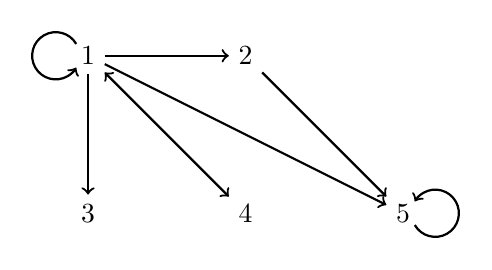
\begin{tikzpicture}
\node (atom1) at (0,2) {1};
\node (atom2) at (2,2) {2};
\node (atom4) at (0,0) {3};
\node (atom5) at (2,0) {4};
\node (atom6) at (4,0) {5};
\draw[->, thick] (atom1)+(-0.15,0.15) arc (-330:-30:.3);
\draw[->, thick] (atom6)+(0.15,-0.15) arc (-150:150:.3);
\draw[->, thick] (atom1) -- (atom2);
\draw[->, thick] (atom1) -- (atom4);
\draw[<->, thick] (atom1) -- (atom5);
\draw[->, thick] (atom1) -- (atom6);
\draw[->, thick] (atom2) -- (atom6);
\end{tikzpicture}
\bmlDescription{Os números 1, 2, 3, 4 e 5 estão conectados por setas.
Há setas de 1 para 2, 3, 4, 5 e para si mesmo; de 2 para 5,
de 5 para si mesmo e de 4 para 1. Não há nenhuma seta saindo de 3.}
\end{center}
Determine se cada uma das seguintes sentenças é verdadeira ou falsa nessa interpretação:
\begin{compactlist}
\item $\exists x\,\atom{R}{x,x}$ \hfill \myanswer{Verdadeiro}
\item $\forall x\,\atom{R}{x,x}$ \hfill \myanswer{Falso}
\item $\exists x \forall y\,\atom{R}{x,y}$ \hfill \myanswer{Verdadeiro}
\item $\exists x \forall y\,\atom{R}{y,x}$ \hfill \myanswer{Falso}
\item $\forall x \forall y \forall z ((\atom{R}{x,y} \eand \atom{R}{y,z}) \eif \atom{R}{x,z})$ \hfill \myanswer{Falso}
\item $\forall x \forall y \forall z ((\atom{R}{x,y} \eand \atom{R}{x,z}) \eif \atom{R}{y,z})$ \hfill \myanswer{Falso}
\item $\exists x \forall y \enot \atom{R}{x,y}$ \hfill \myanswer{Verdadeiro}
\item $\forall x(\exists y\,\atom{R}{x,y} \eif \exists y\,\atom{R}{y,x})$ \hfill \myanswer{Verdadeiro}
\item $\exists x \exists y (\enot x = y \eand \atom{R}{x,y} \eand \atom{R}{y,x})$ \hfill \myanswer{Verdadeiro}
\item $\exists x \forall y(\atom{R}{x,y} \eiff x = y)$ \hfill \myanswer{Verdadeiro}
\item $\exists x \forall y(\atom{R}{y,x} \eiff x = y)$ \hfill \myanswer{Falso}
\item $\exists x \exists y(\enot x = y \eand \atom{R}{x,y} \eand \forall z(\atom{R}{z,x} \eiff y = z))$ \hfill \myanswer{Verdadeiro}
\end{compactlist}

\chapter{Conceitos semânticos}
\setcounter{ProbPart}{0}

\solutions
\problempart
Dada a seguinte interpretação:
\begin{ekey}
	\item[\text{domínio}] pessoas
	\item[\atom{W}{x}] \gap{x} é uma mulher (ou menina)
	\item[\atom{M}{x}] \gap{x} é um homem (ou menino)
	\item[\atom{Y}{x,y}] \gap{x} é mais jovem que \gap{y}
	\item[\atom{O}{x,y}] \gap{x} é descendente de \gap{y}
	\item[d] Dana
	\item[a] Alex
\end{ekey}
expresse as seguintes relações:
\begin{compactlist}
	\item \gap{x} é mais velho que \gap{y} \hfill\myanswer{$\atom{Y}{y,x}$}
	\item \gap{x} é a mãe de \gap{y} \hfill\myanswer{$\atom{O}{y,x}
	\eand \atom{W}{x}$}
	\item \gap{x} e \gap{y} são irmãos (observe que você não pode ser irmão de si mesmo) \hfill\myanswer{$\exists z(\atom{O}{x,z} \eand
	\atom{O}{y,z}) \eand \enot x=y$}

	\item \gap{x} é irmão de \gap{y} \hfill\myanswer{$\exists z(\atom{O}{x,z} \eand
	\atom{O}{y,z}) \eand \enot x=y \eand \atom{M}{x}$}
\end{compactlist}

\problempart
Usando a chave de simbolização do exercício anterior, simbolize as seguintes sentenças:

\begin{compactlist}
	\item Alex e Dana são irmãs. \hfill\myanswer{$\exists z(\atom{O}{a,z} \eand
	\atom{O}{d,z}) \eand \enot a=d \eand \atom{W}{a} \eand \atom{W}{d}$}
	\item Pais são mais velhos que seus filhos.
	\hfill\myanswer{$\forall x\forall y((\atom{O}{x,y} \eand
	\atom{M}{y}) \eif \atom{Y}{x,y})$}
	\item Os pais de Alex têm a mesma idade. \hfill\myanswer{$\forall
	x\forall y((\atom{O}{x,a} \eand
	\atom{O}{y,a}) \eif \enot \atom{Y}{x,y})$}
\end{compactlist}

\chapter{Usando interpretações}\setcounter{ProbPart}{0}

\solutions
\problempart
\label{pr.Contingent}
Mostre que cada uma das seguintes sentenças não é nem uma validade nem uma contradição:
\begin{compactlist}
\item $\atom{D}{a} \eand \atom{D}{b}$

\myanswer{A sentença é verdadeira neste modelo:
\begin{ekey}
	\item[\text{domínio}] Stan
	\item[D(x)] Stan
	\item[a] Stan
	\item[b] Stan
\end{ekey}
E é falsa neste modelo:
\begin{ekey}
	\item[\text{domínio}] Stan
	\item[D(x)] % $\emptyset$
	\item[a] Stan
	\item[b] Stan
\end{ekey}}
\item \leftsolutions\ $\exists x\,\atom{T}{x,h}$

\myanswer{A sentença é verdadeira neste modelo:
\begin{ekey}
	\item[\text{domínio}] Stan
	\item[T(x,y)] \ntuple{Stan, Stan}
	\item[h] Stan
\end{ekey}
E é falsa neste modelo:
\begin{ekey}
	\item[\text{domínio}] Stan
	\item[T(x,y)] % $\emptyset$
	\item[h] Stan
\end{ekey}}

\item $\atom{P}{m} \eand \enot\forall x\,\atom{P}{x}$

\myanswer{	A sentença é verdadeira neste modelo:
\begin{ekey}
	\item[\text{domínio}] Stan, Ollie
	\item[P(x)] Stan
	\item[m] Stan
\end{ekey}
E é falsa neste modelo:
\begin{ekey}
	\item[\text{domínio}] Stan
	\item[P(x)] % $\emptyset$
	\item[m] Stan
\end{ekey}}
\item $\forall z\, \atom{J}{z} \eiff \exists y\,\atom{J}{y}$
\item $\forall x (\atom{W}{x,m,n} \eor \exists y\,\atom{L}{x,y})$
\item $\exists x (\atom{G}{x} \eif \forall y\,\atom{M}{y})$
\item $\exists x (x = h \eand x = i)$
\end{compactlist}

\solutions
\problempart
\label{pr.NotEquiv}
Mostre que os seguintes pares de sentenças não são logicamente equivalentes:
\begin{compactlist}
\item $\atom{J}{a}$, $\atom{K}{a}$

\myanswer{Tornando a primeira sentença verdadeira e a segunda falsa:
\begin{ekey}
	\item[\text{domínio}] $0$
	\item[J(x)] $0$
	\item[K(x)] % $\emptyset$
	\item[a] $0$
\end{ekey}}
\item $\exists x\,\atom{J}{x}$, $\atom{J}{m}$

\myanswer{Tornando a primeira sentença verdadeira e a segunda falsa:
\begin{ekey}
	\item[\text{domínio}] $0$, $1$
	\item[J(x)] $0$
	\item[m] $1$
\end{ekey}}
\item $\forall x\,\atom{R}{x,x}$, $\exists x\,\atom{R}{x,x}$

\myanswer{Tornando a primeira sentença falsa e a segunda verdadeira:
\begin{ekey}
	\item[\text{domínio}] $0$, $1$
	\item[R(x,y)] \ntuple{$0$,$0$}
\end{ekey}}
\item $\exists x\,\atom{P}{x} \eif \atom{Q}{c}$, $\exists x (\atom{P}{x} \eif \atom{Q}{c})$

\myanswer{Tornando a primeira sentença falsa e a segunda verdadeira:
\begin{ekey}
	\item[\text{domínio}] $0$, $1$
	\item[P(x)] $0$
	\item[Q(x)] % $\emptyset$
	\item[c] $0$
\end{ekey}}
\item $\forall x(\atom{P}{x} \eif \enot \atom{Q}{x})$, $\exists x(\atom{P}{x} \eand \enot \atom{Q}{x})$

\myanswer{Tornando a primeira sentença verdadeira e a segunda falsa:
\begin{ekey}
	\item[\text{domínio}] $0$
	\item[P(x)] % $\emptyset$
	\item[Q(x)] % $\emptyset$
\end{ekey}}
\item $\exists x(\atom{P}{x} \eand \atom{Q}{x})$, $\exists x(\atom{P}{x} \eif \atom{Q}{x})$

\myanswer{Tornando a primeira sentença falsa e a segunda verdadeira:
\begin{ekey}
	\item[\text{domínio}] $0$
	\item[P(x)] % $\emptyset$
	\item[Q(x)] $0$
\end{ekey}}
\item $\forall x(\atom{P}{x}\eif \atom{Q}{x})$, $\forall x(\atom{P}{x} \eand \atom{Q}{x})$

\myanswer{Tornando a primeira sentença verdadeira e a segunda falsa:
\begin{ekey}
	\item[\text{domínio}] $0$
	\item[P(x)] % $\emptyset$
	\item[Q(x)] $0$
\end{ekey}}
\item $\forall x\exists y\,\atom{R}{x,y}$, $\exists x\forall y\,\atom{R}{x,y}$

\myanswer{Tornando a primeira sentença verdadeira e a segunda falsa:
\begin{ekey}
	\item[\text{domínio}] $0$, $1$
	\item[R(x,y)] \ntuple{$0$, $1$}, \ntuple{$1$, $0$}
\end{ekey}}
\item $\forall x\exists y\,\atom{R}{x,y}$, $\forall x\exists y\,\atom{R}{y,x}$

\myanswer{Tornando a primeira sentença falsa e a segunda verdadeira:
\begin{ekey}
	\item[\text{domínio}] $0$, $1$
	\item[R(x,y)] \ntuple{$0$, $0$}, \ntuple{$0$, $1$}
\end{ekey}}
\end{compactlist}


\problempart
Mostre que as seguintes sentenças são conjuntamente satisfatíveis:
\begin{compactlist}
\item $\atom{M}{a}, \enot \atom{N}{a}, Pa, \enot \atom{Q}{a}$
\item $\atom{L}{e,e}, \atom{L}{e,g}, \enot \atom{L}{g,e}, \enot \atom{L}{g,g}$
\item $\enot (\atom{M}{a} \eand \exists x\,\atom{A}{x}), Ma \eor \atom{F}{a}, \forall x(\atom{F}{x} \eif \atom{A}{x})$
\item $\atom{M}{a} \eor \atom{M}{b}, \atom{M}{a} \eif \forall x \enot \atom{M}{x}$
\item $\forall y\,\atom{G}{y}, \forall x (\atom{G}{x} \eif \atom{H}{x}), \exists y \enot \atom{I}{y}$
\item $\exists x(\atom{B}{x} \eor \atom{A}{x}), \forall x \enot \atom{C}{x}, \forall x\bigl[(\atom{A}{x} \eand \atom{B}{x}) \eif \atom{C}{x}\bigr]$
\item $\exists x\,\atom{X}{x}, \exists x\,\atom{Y}{x}, \forall x(\atom{X}{x} \eiff \enot \atom{Y}{x})$
\item $\forall x(\atom{P}{x} \eor \atom{Q}{x}), \exists x\enot(\atom{Q}{x} \eand \atom{P}{x})$
\item $\exists z(\atom{N}{z} \eand \atom{O}{z,z}), \forall x\forall y(\atom{O}{x,y} \eif \atom{O}{y,x})$
\item $\enot \exists x \forall y\,\atom{R}{x,y}, \forall x \exists y\,\atom{R}{x,y}$
\item $\enot \atom{R}{a,a}$, $\forall x (x=a \eor \atom{R}{x,a})$

\myanswer{As sentenças são ambas verdadeiras nesta interpretação:
\begin{ekey}
	\item[\text{domínio}] Harry, Sally
	\item[R(x,y)]\ntuple{Sally, Harry}
	\item[a] Harry
	\end{ekey}}
\item $\forall x\forall y\forall z[(x=y \eor y=z )\eor x=z]$, $\exists x\exists y\ \enot x= y$

\myanswer{Não há predicados nem constantes, portanto só precisamos fornecer um domínio. Qualquer domínio com 2 elementos servirá.}

\item $\exists x\exists y((\atom{Z}{x} \eand \atom{Z}{y} )\eand x=y)$, $\enot \atom{Z}{d}$, $d=e$
\end{compactlist}

\problempart
Mostre que os seguintes argumentos são inválidos:
\begin{compactlist}
\item $\forall x(\atom{A}{x} \eif \atom{B}{x}) \therefore \exists x\,\atom{B}{x}$
\item $\forall x(\atom{R}{x} \eif \atom{D}{x}), \forall x(\atom{R}{x} \eif \atom{F}{x}) \therefore \exists x(\atom{D}{x} \eand \atom{F}{x})$
\item $\exists x(\atom{P}{x}\eif \atom{Q}{x}) \therefore \exists x\,\atom{P}{x}$
\item $\atom{N}{a} \eand \atom{N}{b} \eand \atom{N}{c} \therefore \forall x\,\atom{N}{x}$
\item $\atom{R}{d,e}, \exists x\,\atom{R}{xd} \therefore \atom{R}{e,d}$
\item $\exists x(\atom{E}{x} \eand \atom{F}{x}), \exists x\,\atom{F}{x} \eif \exists x\,\atom{G}{x} \therefore \exists x(\atom{E}{x} \eand \atom{G}{x})$
\item $\forall x\,\atom{O}{x,c}, \forall x\,\atom{O}{c,x} \therefore \forall x\,\atom{O}{x,x}$
\item $\exists x(\atom{J}{x} \eand \atom{K}{x}), \exists x \enot \atom{K}{x}, \exists x \enot \atom{J}{x} \therefore \exists x(\enot \atom{J}{x} \eand \enot \atom{K}{x})$
\item $\atom{L}{a,b} \eif \forall x\,\atom{L}{x,b}, \exists x\,\atom{L}{x,b} \therefore \atom{L}{b,b}$
\item $\forall x(\atom{D}{x} \eif \exists y\,\atom{T}{y,x}) \therefore \exists y \exists z\ \enot y= z$
\end{compactlist}

\stepcounter{chapter} % Reasoning about interpretations

\chapter{Propriedades das relações}
\setcounter{ProbPart}{0}

\solutions
\problempart
Dê exemplos de relações com as seguintes propriedades:
\begin{compactlist}
	\item Reflexiva, mas não simétrica \hfill\myanswer{\gap{x} não é mais velho que \gap{y}}

	\item Simétrica, mas não transitiva \hfill\myanswer{\gap{x} está a menos de 1~km de \gap{y}}

	\item Transitiva, simétrica, mas não reflexiva
	\hfill\myanswer{\gap{x} é irmão ou irmã pleno (isto é, não meio-irmão) de \gap{y}}
\end{compactlist}

\problempart
Mostre que uma relação pode ser simultaneamente simétrica e antissimétrica, fornecendo uma interpretação que torne verdadeiras as duas sentenças seguintes:


\begin{align*}
	& \forall x\forall y(\atom{R}{x,y} \eif \atom{R}{y,x})\\
	& \forall x\forall y((\atom{R}{x,y} \eand \atom{R}{y,x}) \eif x=y)
\end{align*}
\myanswer{\begin{ekey}
	\item[\text{domínio}] $0$
	\item[\atom{R}{x,y}] \ntuple{$0$, $0$}
\end{ekey}}
